% -*-latex-*-
%
%  The contents of this file are subject to the University of Utah Public
%  License (the "License"); you may not use this file except in compliance
%  with the License.
%
%  Software distributed under the License is distributed on an "AS IS"
%  basis, WITHOUT WARRANTY OF ANY KIND, either express or implied. See the
%  License for the specific language governing rights and limitations under
%  the License.
%
%  The Original Source Code is SCIRun, released March 12, 2001.
%
%  The Original Source Code was developed by the University of Utah.
%  Portions created by UNIVERSITY are Copyright (C) 2001, 1994
%  University of Utah. All Rights Reserved.
%

\chapter{Working with Networks}
\label{ch:workwithnets}

This section describes how to create, save, load, execute, and edit
networks.

When started with no arguments, the \command{scirun} command creates a
main window with a blank NetEdit frame. The user can create and
connect modules to form a network.

The following conventions are used when describing mouse and keyboard
actions performed by the user:

\begin{description}
\descitem{Button1} Left mouse button

\descitem{Button2} Middle mouse button

\descitem{Button3} Right mouse button

\descitem{Press} ``Press'' means press and hold a key or mouse button.

\descitem{Click} ``Click'' means press and release a key or mouse button.

\descitem{Button\repaceable{N}-Drag} Press and hold Button\repaceable{N},
then drag the mouse.

\descitem{C-Button\repaceable{N}} Press and hold the
\keyboard{Control} key, then press or click Button\repaceable{N}

\descitem{C-\replaceable{key}} Press and hold the control key, then
press key \replaceable{key}
\end{description}


\section{Anatomy of a Module}
\label{sec:modanatomy}

%begin{latexonly}
  \newcommand{\modgraphic}%
  {\centerline{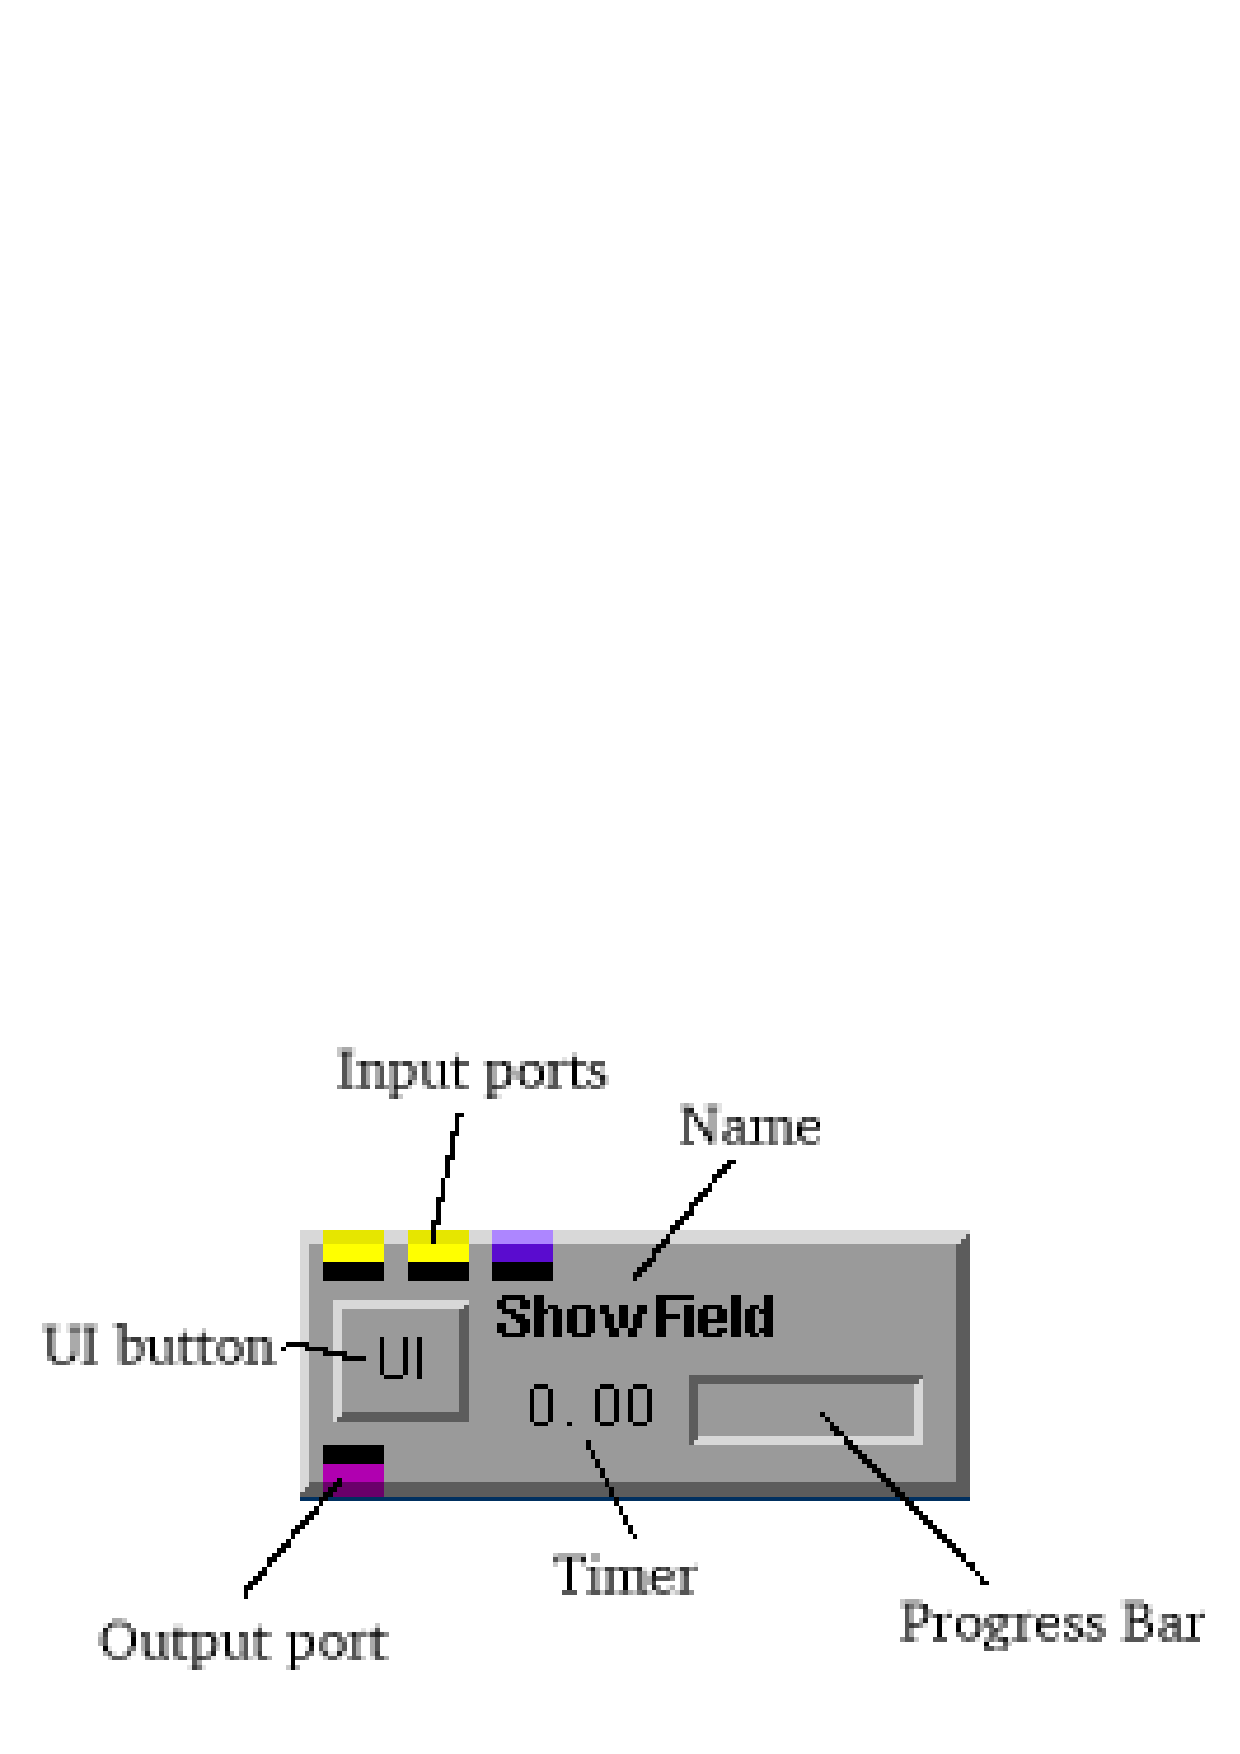
\epsfig{file=Figures/modgraphic-1.eps.gz,width=4in,
        bbllx=0, bblly=0, bburx=325, bbury=157}}}
%end{latexonly}
\begin{htmlonly}
  \newcommand{\modgraphic}{%
  \htmladdimg[align=top,width="256",alt="SCIRun Module Graphic"]
  {../Figures/modgraphic-1.gif}}
\end{htmlonly}

All modules are similarly represented by a graphic within the NetEdit frame
(see Figure~\ref{fig:modgraphic}). The graphical ``front end'' is the same
for all modules and consists of the following elements:

\begin{figure}[htb]
  \begin{makeimage}
  \end{makeimage}
  \modgraphic
  \caption{\label{fig:modgraphic} Module Graphic (\module{Show
      Field} Module)}
\end{figure}

\begin{description}
  \descitem{Module Name} The module's name.
  
  \descitem{Input Ports} Zero or more input ports located on the top
  of the module.  Each port corresponds to a data type and each data
  type has a unique color.  Table~\ref{tab:portcolors} maps port
  colors to data types.  Input ports connect to other modules' output
  ports.  Connections can only be made between ports of the same type.

  \begin{table}[htbp]
    \begin{center}
      \begin{tabular}{|l|l|}
        \hline
        \textbf{Data Type} & \textbf{Port Color} \\
        \hline
        Field & Yellow \\
        Field Set & Green \\
        Matrices & Blue \\
        Geometric Objects & Pink \\
        Color Maps & Purple \\
        Camera Path & Brown \\
        \hline
      \end{tabular}
      \caption{Data Types and their Port Colors}
      \label{tab:portcolors}
    \end{center}
  \end{table}
  
  \descitem{Output ports} Zero or more output ports located on the
  bottom of the module.  Output ports connect to other modules' input
  ports.  Every module has  at least one input or one output
  port.
  
  \descitem{UI button} Pressing the \button{UI} button displays the
  module's control dialog. Some modules have no dialog, some have
  simple dialogs, and some have complex dialogs that allow
  elaborate control over the module.  Figure~\ref{fig:moddialog} shows
  the control dialog for \module{Show Field} module.
  
  \descitem{Progress bar} Shows the module's progress.  As the module
  works toward completion of its task, the progress bar is filled
  with red, then yellow, then green.  When the Progress bar
  is green, the module is done.
  
  \descitem{Timer} Displays the amount of CPU time the module has
  consumed.  Located to the left of the progress bar.
  
  \descitem{Message Indicator} Shows the presence of messages in a
  module's log.  Colors represent message types.  Blue represents
  ``remarks'' (informational messages) and yellow represents ``warnings''
  (attention is needed).  Click the indicator to display the
  module's log.
  
  \descitem{Pop-up Menu} Pressing Button3 while the mouse pointer is
  over a module activates a module's pop-up menu.  The content
  of the pop-up menu changes depending on the state of the NetEdit
  window. The following items are available in the pop-up menu:

  \begin{description}
    \menuitemdesc{::Package\_Category\_Name\_Instance} This item is a
    label (not a selectable item).  It provides the module's name and
    the category and package to which the module belongs.
    ``Instance'' is a unique number that distinguishes multiple
    instances of the same module.
    
    \menuitemdesc{Execute} Tells the module to execute (or
    re-execute).  This may cause other modules in the network to
    execute or``fire'' (see \secref{Executing a
      Network}{sec:executenet}).

    \menuitemdesc{Help} Displays the module's help window.
    
    \menuitemdesc{Notes} Displays a module's note pad.  The note pad
    is used to document the purpose of a module in a network.  See
    \secref{Displaying Module Notes}{sec:modnotes}.

    \menuitemdesc{Destroy Selected} Destroys the selected modules.
    See \secref{Destroying Module(s)}{sec:destroymod}.
    
    \menuitemdesc{Destroy} Destroys the module See \secref{Destroying
      Module(s)}{sec:destroymod}.
    
    \menuitemdesc{Show Log} Displays the module's message log.  Most
    modules write messages to their log during the course of
    their execution (see \secref{Viewing a Module's Log}{sec:viewmodslog}).
    
    \menuitemdesc{Make Sub-Network} Creates a sub-network from
    selected modules.  See \secref{Creating a Sub-Network}{sec:subnet}.
    
    \menuitemdesc{Expand Sub-Network} Reverses the action of menu item
    \menuitem{Make Sub-Network}.  This menu item is available only in
    a sub-network's pop-up menu.  See \secref{Expanding a
      Sub-Network}{sec:subnet}.
    
    \menuitemdesc{Disable} Disables a module.  See
    \secref{Disabling/Enabling Modules}{sec:disablemod}.
    
    \menuitemdesc{Enable} Enables a disabled module.  See
    \secref{Disabling/Enabling Modules}{sec:disablemod}.

  \end{description}
\end{description}


\section{Anatomy of a Connection}
\label{sec:anatcon}

A connection lets data flow from one module's output port to (usually) another
module's input port.  Sometimes a connection will connect a module's
output port to its input port.

Connections are colored differently if they are enabled or disabled.

Pressing \keyboard{Button3} while the mouse pointer is over a connection
activates a connection's pop-up menu.  The content of the pop-up menu
changes depending on the state of the connection. The following items are
available in the pop-up menu:

\begin{description}
  \menuitemdesc{Delete} Deletes a connection.
  
  \menuitemdesc{Disable} Disables a connection.
  
  \menuitemdesc{Enable} Enables a disabled connection.

  \menuitemdesc{Notes} Displays a connection's note pad.
\end{description}

\section{Creating a Module}
\label{sec:creatingmodules}

To create a module, select its name from one of the package (\eg{}
\sr) menus' category sub-menus. Package menus are accessed from the
main window's menu bar or from the NetEdit frame's pop-up menu.  The
NetEdit frame's pop-up menu is activated by pressing
\keyboard{Button3} (right mouse button) while the mouse pointer is in
the NetEdit frame (but not over a module or connection).  The pop-up
menu contains a list of category sub-menus from the \sr{} package and
other installed packages.  Each category sub-menu provides access to
modules within the category.

After creating a module, its glyph (or graphic representation) is 
placed in the NetEdit frame.

\section{Setting Module Properties}
\label{sec:setmodprops}

%begin{latexonly}
  \newcommand{\moddialog}%
  {\centerline{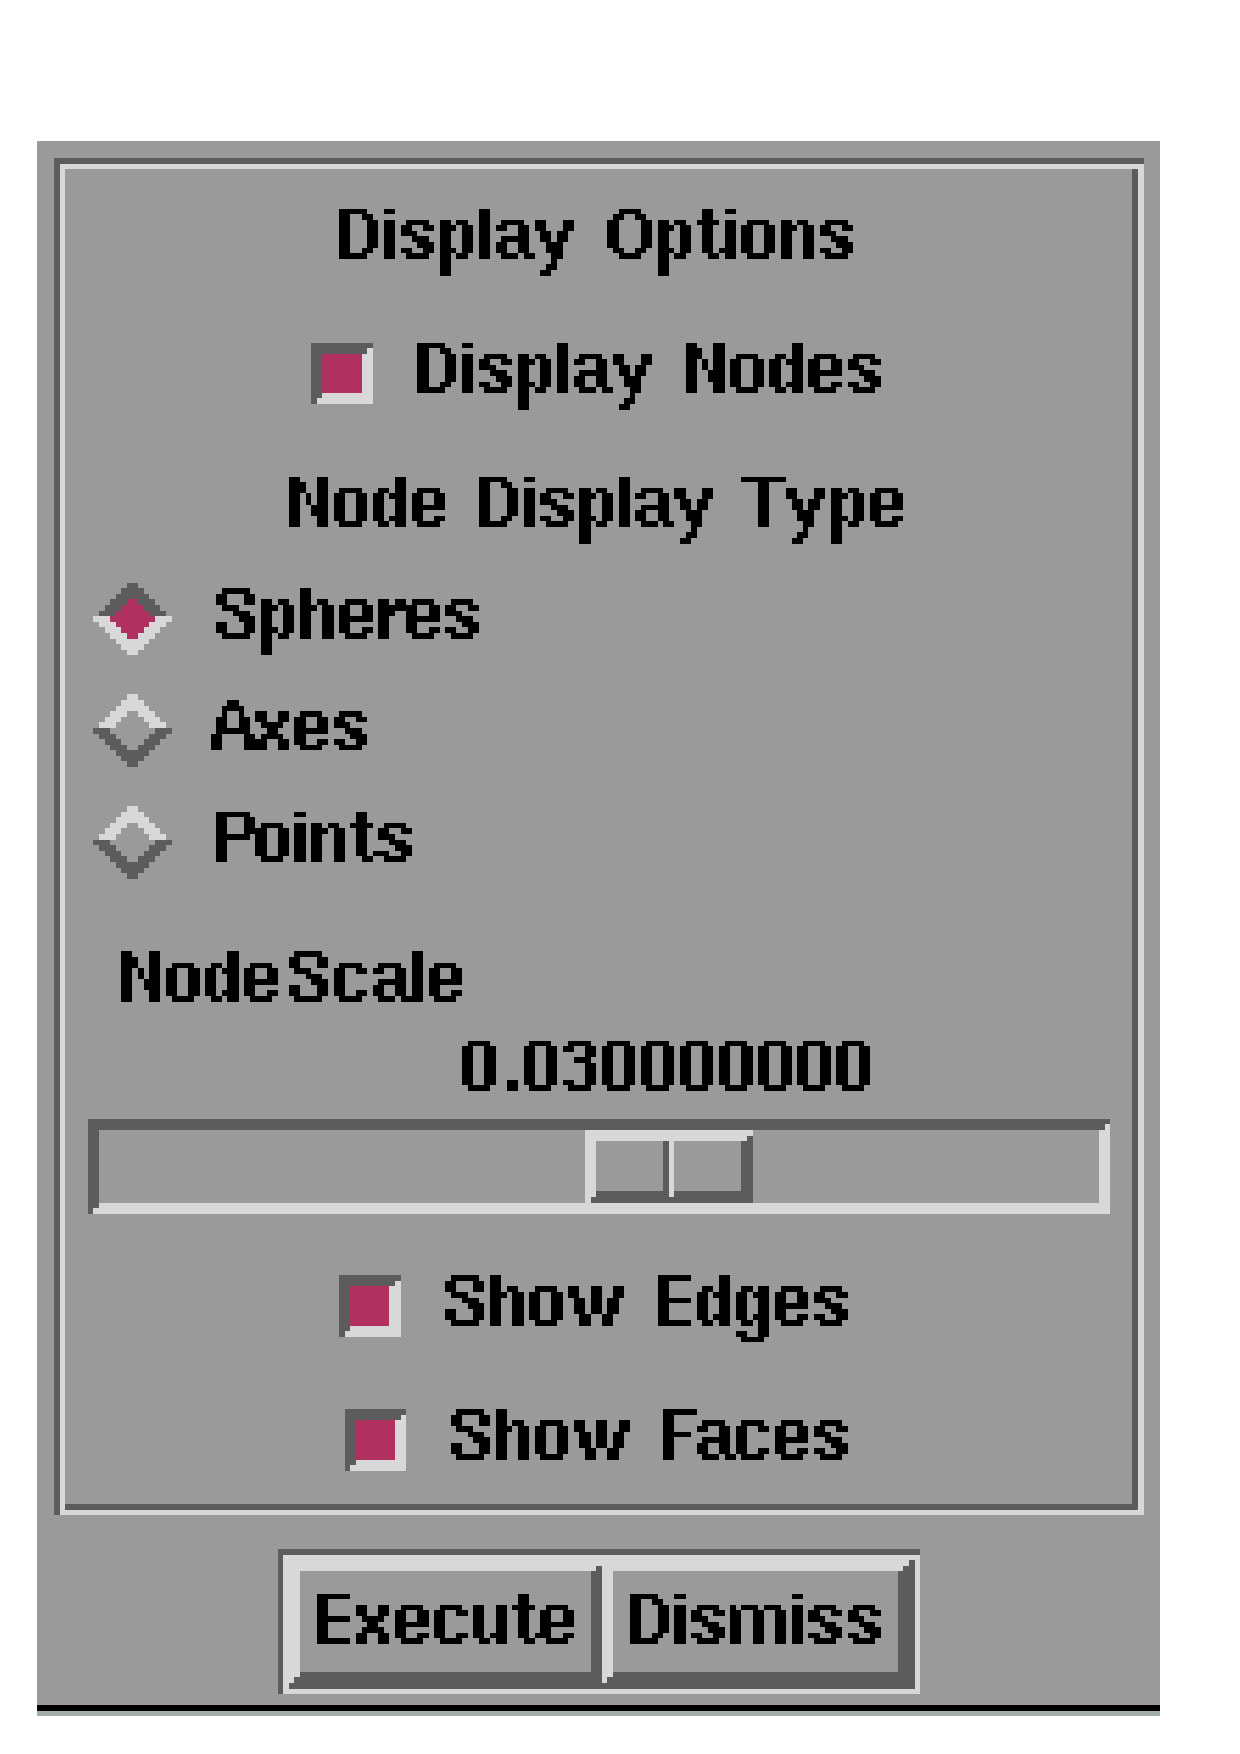
\epsfig{file=Figures/moddialog.eps.gz,
        bbllx=0, bblly=0, bburx=272, bbury=406}}}
%end{latexonly}
\begin{htmlonly}
  \newcommand{\moddialog}{%
  \htmladdimg[align=top,alt="SCIRun Module Dialog"]
  {../Figures/moddialog.gif}}
\end{htmlonly}

To change a module's properties, click its \button{UI} button.  This
displays the module's control dialog.  Use the dialog to change the
module's properties.  Each \htmladdnormallinkfoot{module's reference
  documentation}{\latexhtml{http://software.sci.utah.edu/doc/}{../../../}Developer/Modules/index.html}
explains the use of its control dialog.  Figure~\ref{fig:moddialog}
shows the control dialog for the \module{Show Field} module.

\begin{figure}[htb]
  \begin{makeimage}
  \end{makeimage}
  \moddialog
  \caption{\label{fig:moddialog} Module \module{Show Field}'s Control Dialog
    (User Interface).}
\end{figure}

\section{Selecting Modules}
\label{sec:selectmods}

Some operations (moving, destroying, disabling, and enabling) act on a group of
modules (see \secref{Moving Module(s)}{sec:movemod},
\secref{Destroying Module(s)}{sec:destroymod}, and \secref{Disabling  
Modules}{sec:disablemod}).  A group of modules can be created in
two ways:

\begin{enumerate}
\item Perform \keyboard{Button1-Drag} while the pointer is in the
  NetEdit frame, but not over a module or a connection. This starts a
  selection box, allowing the user to select multiple modules. Only
  modules overlapping the selection box are selected. Release Button1
  to complete the selection.
  
\item Select the first module by clicking \keyboard{Button1} while the
  pointer is over a module.  Then add modules to the group by clicking
  \keyboard{C-Button1} on additional modules.  All previously selected
  modules remain selected.
\end{enumerate}

Selected modules are colored differently from unselected modules.

Modules can be added or removed from a group by pressing the
\keyboard{Control} key while making selections using the above
methods.  If the \keyboard{Control} key is not pressed, the previous
group is forgotten and a new group is created.

\section{Destroying Modules}
\label{sec:destroymod}

To delete a module, choose menu item \menuitem{Destroy} from a module's
pop-up menu.

Multiple modules can be deleted at one time. Select one or more
modules, then choose menu item \menuitem{Destroy} from a module's
pop-up menu.

\section{Moving Modules}
\label{sec:movemod}

Modules can be moved in the NetEdit frame.  To move a module, perform
Button1-Drag while the pointer is over a module, and move the module
to its new location.

Multiple modules can be moved at one time.  Select one or more
modules, then perform Button1-Drag while the pointer is over any one
of the modules in the selected group.

\section{Disabling and Enabling Modules}
\label{sec:disablemod}

Modules may be temporarily disabled.  Disabled modules do not execute
and data does not flow through them.

To disable modules, select one or more modules, then
choose menu item \menuitem{Disable} from a module's pop-up menu.

Disabling a module disables all incoming and outgoing connections to
the module and prevents the module from executing during execution of
the network. Disabled modules are drawn in a darker shade of grey.

To enable disabled modules, choose \menuitem{Enable} from a disabled
module's pop-up menu.  Enabling one module enables all modules in a
disabled module's group.

See also \secref{Disabling/Enabling Connections}{sec:disableconnect}.

\section{Creating a Sub-Network}
\label{sec:crsubnet}

A sub-network is a group of modules that are treated as a single
module.  In a network, you may use a sub-network as you would a
module.

To create a sub-network, select one or more modules, then choose item
\menuitem{Create Sub-Network} from any selected module's pop-up menu.
Selected modules will be replaced by a sub-network graphic and the
sub-network editor will activate.  Sub-networks may be created in
sub-networks.  The next section (\secref{Editing a
  Sub-Network}{sec:editsubnet}) explains the use of the sub-network
editor.

In a sub-network graphic, the CPU time and Progress Bar are
replaced by the \guibutton{Sub-Network} button.  The sub-network
editor is activated by pressing button \guibutton{Sub-Network}.
Pressing button \guibutton{UI} activates control dialogs for all
modules in the sub-network.  Control dialogs can be activated
individually in the sub-network editor.


\section{Editing a Sub-Network}
\label{sec:editsubnet}

The sub-network editor works similarly to the NetEdit window.  All
network editing features of the NetEdit window are available in the
sub-network editor.  The sub-network editor is activated by pressing a
sub-network's \guibutton{Sub-Network} button.

In addition, sub-networks can have input and output ports and these
can be created in the sub-network editor.  Sub-network input ports can
be created by making a connection between the input port of a module
(a module in the sub-network) and the top edge of the sub-network
editor window.  Sub-network output ports can be created by making a
connection between the output port of a module (a module in the
sub-network) and the bottom edge of the sub-network editor window.

A sub-network can be renamed by entering the new name into the text
entry widget labeled \guilabel{Name}.

%% \section{Saving and Reusing Sub-Networks}
%% \label{sec:savesubnet}

%% A sub-network can be saved for reuse in other networks or
%% sub-networks.  To save a sub-network, activate the sub-network by
%% pressing its \guibutton{Sub-Network} button, then press button
%% \guibutton{Save}.

%% A sub-network can be reused by 

\section{Expanding a Sub-Network}
\label{sec:expsubnet}

Expanding a network reverses the action of menu item \menuitem{Create
  Sub-Network}.  To expand a sub-network choose menu item
\menuitem{Expand Sub-Network} from the sub-network's pop-up menu.
  This action cannot be ``undone.''


\section{Editing and Displaying Module Notes}
\label{sec:modnotes}

Module notes allow the user to document the purpose of
each module by attaching notes to each module in the NetEdit window.
Notes can be displayed or hidden.

To create or edit module notes, choose menu item \menuitem{Notes} from
a module's pop-up menu. Enter new notes or edit existing notes in
the note editor dialog.

Notes may be hidden, displayed in \dfn{tooltips}, or displayed in the
NetEdit window.  The note editor provides the following note display
options: \guibutton{Default}, \guibutton{Tooltip}, \guibutton{Top},
\guibutton{Left}, \guibutton{Right}, or \guibutton{Bottom}.  Choose a
display mode by clicking \keyboard{Button1} on the appropriate button.

Choose \guibutton{tooltips} to display notes as tooltips.  Notes are
displayed only when the mouse pointer hovers over a module.

Choose one of \guibutton{Default}, \guibutton{Top}, \guibutton{Left},
\guibutton{Right}, or \guibutton{Bottom} to display notes in the
NetEdit to the right, top, left, right, or bottom of the module
respectively. 

Choose \guibutton{None} to hide module notes.  Displayed notes can be
hidden by clicking \keyboard(Button2) when the pointer is on the
notes.  Hiding notes does not delete notes.

The note editor dialog can be activated by clicking \keyboard{Button1}
on notes displayed in the NetEdit window.


\section{Viewing a Module's Log}
\label{sec:viewmodslog}

Each module supports a message log. The module writes error messages
or other types of messages to its log.

To display a modules log, choose \menuitem{Show Log} from a module's
pop-up menu.


\section{Creating a Connection}
\label{sec:connectmods}

To connect the output (input) port of one module to the input (output)
port of another module, use \keyboard(Button2). Clicking \keyboard(Button3) on a connection
gives access to a pop-up menu. Use the pop-up menu to disable, delete,
or annotate a connection.

To make a connection, position the mouse pointer over a module's input
(output) port.  Then perform \keyboard{Button2-Drag} and drag the
mouse pointer toward another module's output (input) port.

When \keyboard(Button2) is pressed, the program shows all valid connections as black
lines.  It also draws one red colored connection, which is the
connection made if the drag is stopped by releasing \keyboard(Button2).

Make the connection by releasing \keyboard(Button2) when the pointer is over the
desired destination port, or when the red colored connection is the
desired connection.  The connection is drawn using the color
corresponding to the connection's data type.

Users can connect a module's output port to the input ports of one or more
modules by repeating the procedure just described.

\section{Editing/Displaying Connection Notes}
\label{sec:displaynotes}

Connection notes allow the user to document the purpose of
each connection by attaching notes to each connection in the NetEdit window.
Notes can be displayed or hidden.

To create or edit connection notes, choose menu item \menuitem{Notes} from
a connection's pop-up menu. Enter new notes or edit existing notes in
the note editor dialog.

Notes may be hidden, displayed in \dfn{tooltips}, or displayed in the
NetEdit window.  The note editor provides the following note display
options: \guibutton{Default}, \guibutton{Tooltip}, \guibutton{Top},
\guibutton{Left}, \guibutton{Right}, or \guibutton{Bottom}.  Choose a
display mode by clicking \keyboard{Button1} on the appropriate button.

Choose \guibutton{tooltips} to display notes as tooltips.  Notes are
displayed only when the mouse pointer hovers over a connection.

Choose one of \guibutton{Default}, \guibutton{Top}, \guibutton{Left},
\guibutton{Right}, or \guibutton{Bottom} to display notes in the
NetEdit to the right, top, left, right, or bottom of the connection
respectively. 

Choose \guibutton{None} to hide connection notes.  Displayed notes can be
hidden by clicking \keyboard(Button2) when the pointer is over the
notes.  Hiding notes does not delete notes.

The note editor dialog can be activated by clicking \keyboard{Button1}
on notes displayed in the NetEdit window.

\section{Highlighting Related Connections}
\label{sec:highlightconnect}

To highlight the tree of connections affecting a connection, click
\keyboard(Button1) anywhere on a connection.

To highlight the tree of connections downstream an output port,
click \keyboard(Button1) on the output port.

To highlight the tree of connections upstream an input port,
click \keyboard(Button1) on the input port.

\section{Disabling a Connection}
\label{sec:disableconnect}

To disable a connection, click \keyboard(Button3) on the connection to
bring up the connection menu and select \menuitem{Disable}. The
connection appears grey.

Disabling a connection blocks data from flowing through, as if it were
not connected.

\section{Undoing/Redoing a Connection}
\label{sec:undomod}

Type \keyboard{C-z} to undo the last connection creation or deletion.
Undo can be repeated.

Type \keyboard{C-y} to redo the last undone connection creation or
deletion.
 
\section{Deleting a Connection}
\label{sec:deleteconnections}

To delete a connection, choose menu item \menuitem{Delete} from a
connection's pop-up menu or click \keyboard{C-Button2} while the
pointer is on a connection.

\section{Executing a Network}
\label{sec:executenet}

``Network Execution'' means one or more modules must be executed in a
coordinated fashion. 
\sr{}'s \dfn{scheduler} manages the coordinated execution of modules.

Note that some modules need to be compiled before they are
executed (see \secref{Dynamic Compilation}{sec:dyncomp}).  Compilation
delays execution of the network.  This delay occurs only one time
(per module).  After a module is compiled, it does not need to be
compiled again.  Modules change color during compilation.

\subsection{The Basics}

The scheduler is invoked when an event \dfn{triggers} a
module's execution.  The scheduler creates a list of all modules that
must execute in coordination with the triggered module. Modules
\dfn{upstream} (directly or indirectly) from the triggered module are 
put on the execution list if they have not previously executed.
All modules \dfn{downstream} from the triggered module are put
on the execution list.  Once the scheduler determines which modules must be
executed, it executes them (in parallel where possible).

Network execution is mostly transparent.  That is, events that trigger
module execution usually generate automatically. Sometimes,
however, the user must manually
generate a triggering event by choosing the \menuitem{Execute} item from a
module's pop-up menu.

\subsection{Details}

Each module executes in its own thread and blocks (waits) until its upstream
modules can supply it with data.  After a module completes its computation,
it sends the results to its downstream modules.  This completes a module's
execution cycle.  The module will not have another chance to receive data from its input ports
and send data to its output ports until some event
puts the  module back on the scheduler's execution list.  

This behavior prevents modules from computing in an iterative fashion 
(sending intermediate results to their downstream modules), because
downstream modules cannot receive results until they are in their
execution cycle. Downstream modules would need to be executed each time the
upstream module posts an intermediate result.


\subsection{Intermediate Results}

Some modules are designed to be used in an iterative fashion. They use
a method called \icode{send\_intermediate} to send the results of each
iteration.  When this method is used, the scheduler (re)executes
downstream modules each time the upstream module posts its next
result.  Downstream modules are able to receive the results of each
iteration as soon as the upstream module sends them.

Modules \module{SolveMatrix} and \module{MatrixSelectVector} (from the
\package{\sr} package and \category{Math} category) are examples of modules
that compute iteratively using the \icode{send\_intermediate} method.

\subsection{Feedback Loops}

Some modules are designed to be used exclusively in feedback
loops. Their output ports can be connected
directly or indirectly to their input ports.  These modules also use the
\icode{send\_intermediate} method.

Examples of feedback modules are \module{DipoleSearch} and
\module{ConductivitySearch} from the \category{Inverse} category of the
\package{BioPSE} package and \module{BuildElemLeadField} from the
\category{LeadField} category of the \package{BioPSE} package.

\section{Documenting a Network}
\label{sec:docnetwork}

It is useful to document the function of a network.  A network's note
pad is used for this purpose.  To edit the network's note pad,
select the \menuitem{Add Info} item from the main window's \menu{File}
menu.  This displays the network's note pad editor.  The editor
allows the user to write notes on the purpose and use of the network.

\section{Saving a Network}
\label{sec:savenet}

\sr{} can save networks to files.  Network files have an extension of
\filename{.net} (in the past they also had .sr and .uin
extensions).  

To save a network, select \menuitem{Save} item from the main window's
\menu{File} menu.  A file browser dialog prompts for the
name and location of the network file.

If  changes are made to an existing network, \menuitem{Save} 
saves changes made to an existing net file.

Save an existing network under a new name using the
\menuitem{Save As...} menu item.  A file browser dialog prompts
for the new name of the network file.  Subsequent uses of
\menuitem{Save} saves changes to the newly created file.

Network files are  \dfna{Tool Command Language}{TCL} scripts.
These files can be edited, however, reasons for doing so are beyond
the scope of this guide.

\section{Loading a Network}
\label{sec:opennet}

To load a network file, select the \menuitem{Load} item from the main
window's \menu{File} menu.   A file browser dialog prompts for the
name and location of the network file.

Note that loading a network file adds the network to an existing network in
the NetEdit frame, possibly overlapping the networks.

\section{Inserting a Network}
\label{sec:insertnetwork}

To avoid merging networks, select the
\menuitem{Insert} item from the main window's \menu{File} menu. This
option allows the user to place one \sr{} network next to another,
avoiding overlap.  A file browser dialog prompts the user for the name and
location of the network file.

The new network is inserted into the upper left corner of the
NetEdit frame.  If a network of modules already exists in the NetEdit
frame, the \menuitem{Insert} command places a new network to the
immediate right of the existing network.

\section{Clearing a Network}
\label{sec:clearnetwork}

To remove all modules and connections from the 
NetEdit frame, select the \menuitem{Clear} item from the main window's
\menu{File} menu.  A text box appears, confirming whether the
user wants to proceed with or cancel the clearing operation.

\section{Navigating a Network}
\label{sec:navnetwork}

A complex network may not be entirely visible in the NetEdit frame.
Use the NetEdit frame's scroll bars or the network view tool to view
complex networks.

The Global View Frame shows the entire ``network world.''  The small
rectangular region (outlined in black) in the Global View Frame is the
network view tool and a window on the network world. The position of
the view tool determines the part of the network visible in the
NetEdit frame.  To view other parts of the network, press
\keyboard(Button1) while the pointer is anywhere in the Global View
Frame---this moves the tool to the location of the pointer -- then
drag the tool to the new location.


\section{The \sr{} Shell}
\label{sec:termapp}

After starting, \sr{} runs a shell-like application in the terminal
window. This shell displays the prompt
\screen{scirun\ra} in the terminal window.This program is a
\dfna{Tool Command Language}{TCL} shell program extended with
\sr{} specific commands.

It is possible to type \tcl{} \sr{} commands at the prompt.  For
instance, to load a network type \keyboard{source 
\ptext{network file name}}.  This has the same effect as the \menu{File}
menu's \menuitem{Load} command.
